\section{Teoretični model}
\subsection{Izpeljava valovne enačbe}

V sklopu predavanj predmeta Matematična fizika 2 smo izpeljali valovno enačbo za struno. Izpeljavo bom tukaj ponovno povzel zaradi celovitosti naloge.

Vrv dolžine \( L \) s konstantno dolžinsko gostoto \( \mu \) visi s stropa, kakor prikazuje slika \ref{fig:koordinate}. Odmiki vrvi naj bodo majhni glede na koordinatno os \( x \) in pravokotni nanjo (naša slika je torej močno pretirana).

\begin{figure}[htbp]
\centerline{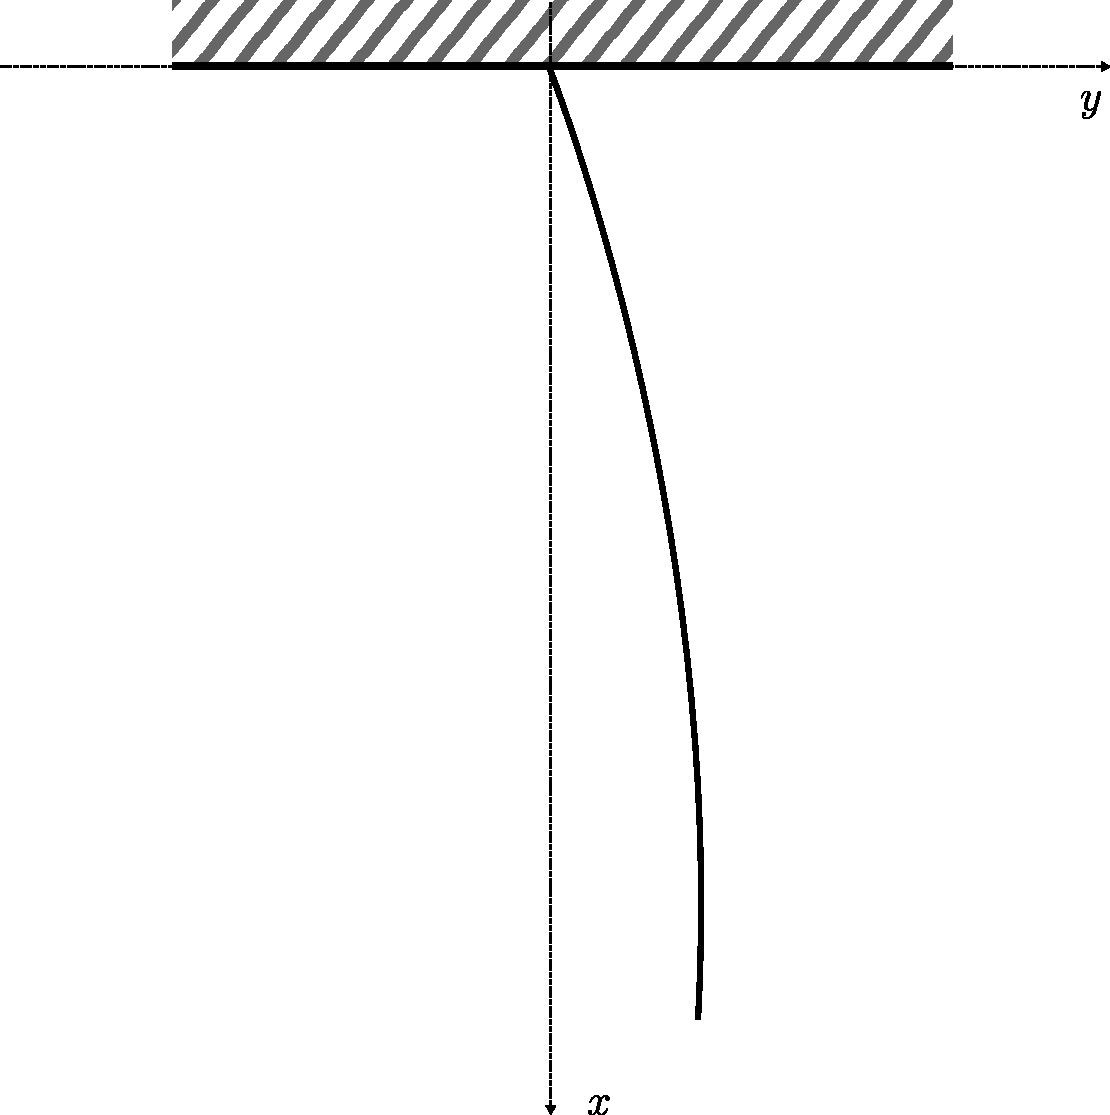
\includegraphics[width=0.45\textwidth]{figures/koordinate.pdf}}
\caption{\small Skica našega problema - težka vrv, ki visi s stropa.\label{fig:koordinate}}
\end{figure}

Opazujemo košček vrvi dolžine \( \mathrm{d} s \) in sile, ki delujejo na njega, kot je prikazano na sliki \ref{fig:koscekVrvi}.

\begin{figure}[htbp]
\centerline{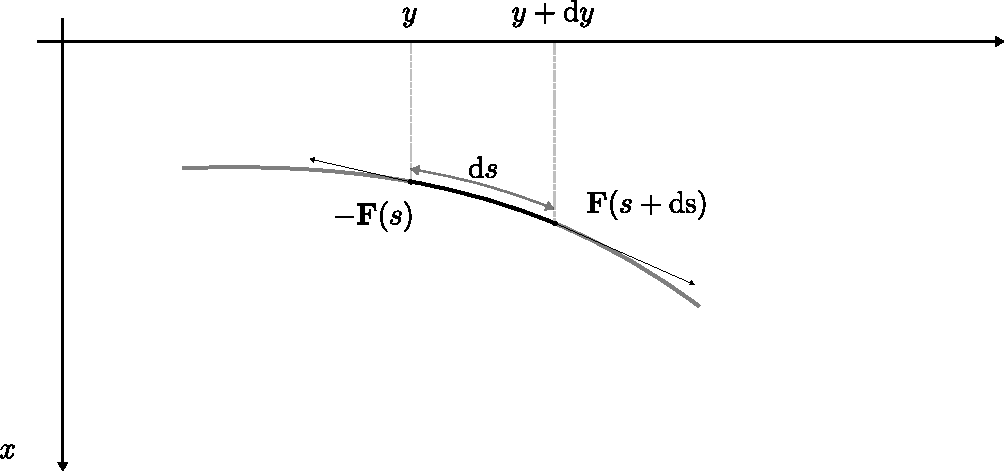
\includegraphics[width=0.60\textwidth]{figures/delcekvrvi.pdf}}
\caption{\small Košček vrvi \( \mathrm{d} s \) in sile, ki delujejo na njega. \label{fig:koscekVrvi}}
\end{figure}

Edina zunanja sila, ki deluje na vrv, je sila teže \( F_x = \mu (L - x) g \). Preko definicije kosinusa zapišemo

\[ F_y = F \frac{\mathrm{d} y}{\mathrm{d} s}. 
\]
Ker so odmiki v smeri \( x \) majhni (\( \mathrm{d} x \ll \mathrm{d} y \)), lahko dolžino loka \( \mathrm{d} s \) nadomestimo s projekcijo \( \mathrm{d} y \). Enako lahko storimo tudi z razliko nateznih sil

\[ \mathbf{F}(s + \mathrm{d}s) - \mathbf{F}(s) = \frac{\partial }{\partial s} F_x = \frac{\partial }{\partial s} \left( F \frac{\mathrm{d} x}{\mathrm{d} s} \right).
\]
Razlika nateznih sil po drugem Newtonovem zakonu struno pospešuje, zato zapišemo

\[ \mu \frac{\partial ^2 y}{\partial t ^2} = \frac{\partial }{\partial s} \left( F \frac{\mathrm{d} x}{\mathrm{d} s} \right)  
\]


\subsection{Definicija problema}
\subsection{Splošna rešitev}
\subsection{Začetni pogoji}
